%% Creator: Inkscape 0.48.3.1, www.inkscape.org
%% PDF/EPS/PS + LaTeX output extension by Johan Engelen, 2010
%% Accompanies image file 'CatMapStatesp.pdf' (pdf, eps, ps)
%%
%% To include the image in your LaTeX document, write
%%   \input{<filename>.pdf_tex}
%%  instead of
%%   \includegraphics{<filename>.pdf}
%% To scale the image, write
%%   \def\svgwidth{<desired width>}
%%   \input{<filename>.pdf_tex}
%%  instead of
%%   \includegraphics[width=<desired width>]{<filename>.pdf}
%%
%% Images with a different path to the parent latex file can
%% be accessed with the `import' package (which may need to be
%% installed) using
%%   \usepackage{import}
%% in the preamble, and then including the image with
%%   \import{<path to file>}{<filename>.pdf_tex}
%% Alternatively, one can specify
%%   \graphicspath{{<path to file>/}}
%% 
%% For more information, please see info/svg-inkscape on CTAN:
%%   http://tug.ctan.org/tex-archive/info/svg-inkscape
%%
\begingroup%
  \makeatletter%
  \providecommand\color[2][]{%
    \errmessage{(Inkscape) Color is used for the text in Inkscape, but the package 'color.sty' is not loaded}%
    \renewcommand\color[2][]{}%
  }%
  \providecommand\transparent[1]{%
    \errmessage{(Inkscape) Transparency is used (non-zero) for the text in Inkscape, but the package 'transparent.sty' is not loaded}%
    \renewcommand\transparent[1]{}%
  }%
  \providecommand\rotatebox[2]{#2}%
  \ifx\svgwidth\undefined%
    \setlength{\unitlength}{97.83133397bp}%
    \ifx\svgscale\undefined%
      \relax%
    \else%
      \setlength{\unitlength}{\unitlength * \real{\svgscale}}%
    \fi%
  \else%
    \setlength{\unitlength}{\svgwidth}%
  \fi%
  \global\let\svgwidth\undefined%
  \global\let\svgscale\undefined%
  \makeatother%
  \begin{picture}(1,0.81984366)%
    \put(0,0){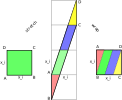
\includegraphics[width=\unitlength]{CatMapStatesp.pdf}}%
    \put(0.02954802,0.1649001){\color[rgb]{0,0,0}\makebox(0,0)[lb]{\smash{A}}}%
    \put(0.26669086,0.17307744){\color[rgb]{0,0,0}\makebox(0,0)[lb]{\smash{B}}}%
    \put(0.26669086,0.41839762){\color[rgb]{0,0,0}\makebox(0,0)[lb]{\smash{C}}}%
    \put(0.02137069,0.41839762){\color[rgb]{0,0,0}\makebox(0,0)[lb]{\smash{D}}}%
    \put(0.38935094,0.00135332){\color[rgb]{0,0,0}\makebox(0,0)[lb]{\smash{B}}}%
    \put(0.38935094,0.21396414){\color[rgb]{0,0,0}\makebox(0,0)[lb]{\smash{A}}}%
    \put(0.64284833,0.60647641){\color[rgb]{0,0,0}\makebox(0,0)[lb]{\smash{C}}}%
    \put(0.64284833,0.79455521){\color[rgb]{0,0,0}\makebox(0,0)[lb]{\smash{D}}}%
    \put(0.79004043,0.42657495){\color[rgb]{0,0,0}\makebox(0,0)[lb]{\smash{A}}}%
    \put(0.79004043,0.17307744){\color[rgb]{0,0,0}\makebox(0,0)[lb]{\smash{B}}}%
    \put(0.96994189,0.17307744){\color[rgb]{0,0,0}\makebox(0,0)[lb]{\smash{C}}}%
    \put(0.97811923,0.42657495){\color[rgb]{0,0,0}\makebox(0,0)[lb]{\smash{D}}}%
    \put(0.1469525,0.17504358){\color[rgb]{0,0,0}\makebox(0,0)[lb]{\smash{x_i}}}%
    \put(-0.00023957,0.29770375){\color[rgb]{0,0,0}\makebox(0,0)[lb]{\smash{x_i}}}%
    \put(0.36774069,0.30588109){\color[rgb]{0,0,0}\makebox(0,0)[lb]{\smash{x_i}}}%
    \put(0.51493279,0.17504367){\color[rgb]{0,0,0}\makebox(0,0)[lb]{\smash{x_i}}}%
    \put(0.86655824,0.16686633){\color[rgb]{0,0,0}\makebox(0,0)[lb]{\smash{x_i}}}%
    \put(0.73572082,0.30588109){\color[rgb]{0,0,0}\makebox(0,0)[lb]{\smash{x_i}}}%
    \put(0.21762677,0.55482852){\color[rgb]{0,0,0}\rotatebox{43.35476392}{\makebox(0,0)[lb]{\smash{stretch}}}}%
    \put(0.74915379,0.61465381){\color[rgb]{0,0,0}\rotatebox{-46.94301089}{\makebox(0,0)[lb]{\smash{wrap}}}}%
  \end{picture}%
\endgroup%
